For each TEC series like figure \ref{fig:detrending-example} we computed $|W_n(s)|^2$ to find any wave-like features in any of the TEC series, where $s$ is the wavelet scale (somehow is the analogous to the wavelength). The presence of this features allow us to trace the TEC perturbations produced by the meteor. Examples are shown in figure \ref{fig:power-spectrums}. Due to the fact we are working with finite time series, edge effects become important at the beginning or the end of the time series, and when the wavelet scale is similar or greater than the time series length. The limit when these errors become important is called Cone of Influence (COI), the COI is shown as a white dashed line in figure \ref{fig:power-spectrums}. At a closer look of this spectra is clear that in some cases the wavelet spectra in the previous day is more intense than the event day. This happens because no TEC perturbations was really detected, but instead noise appears as wavelets. This is an indicator that the TEC perturbances either propagate to other location or it is too faint to be detectable.


\begin{figure*}
  \begin{tabular}{cc}
  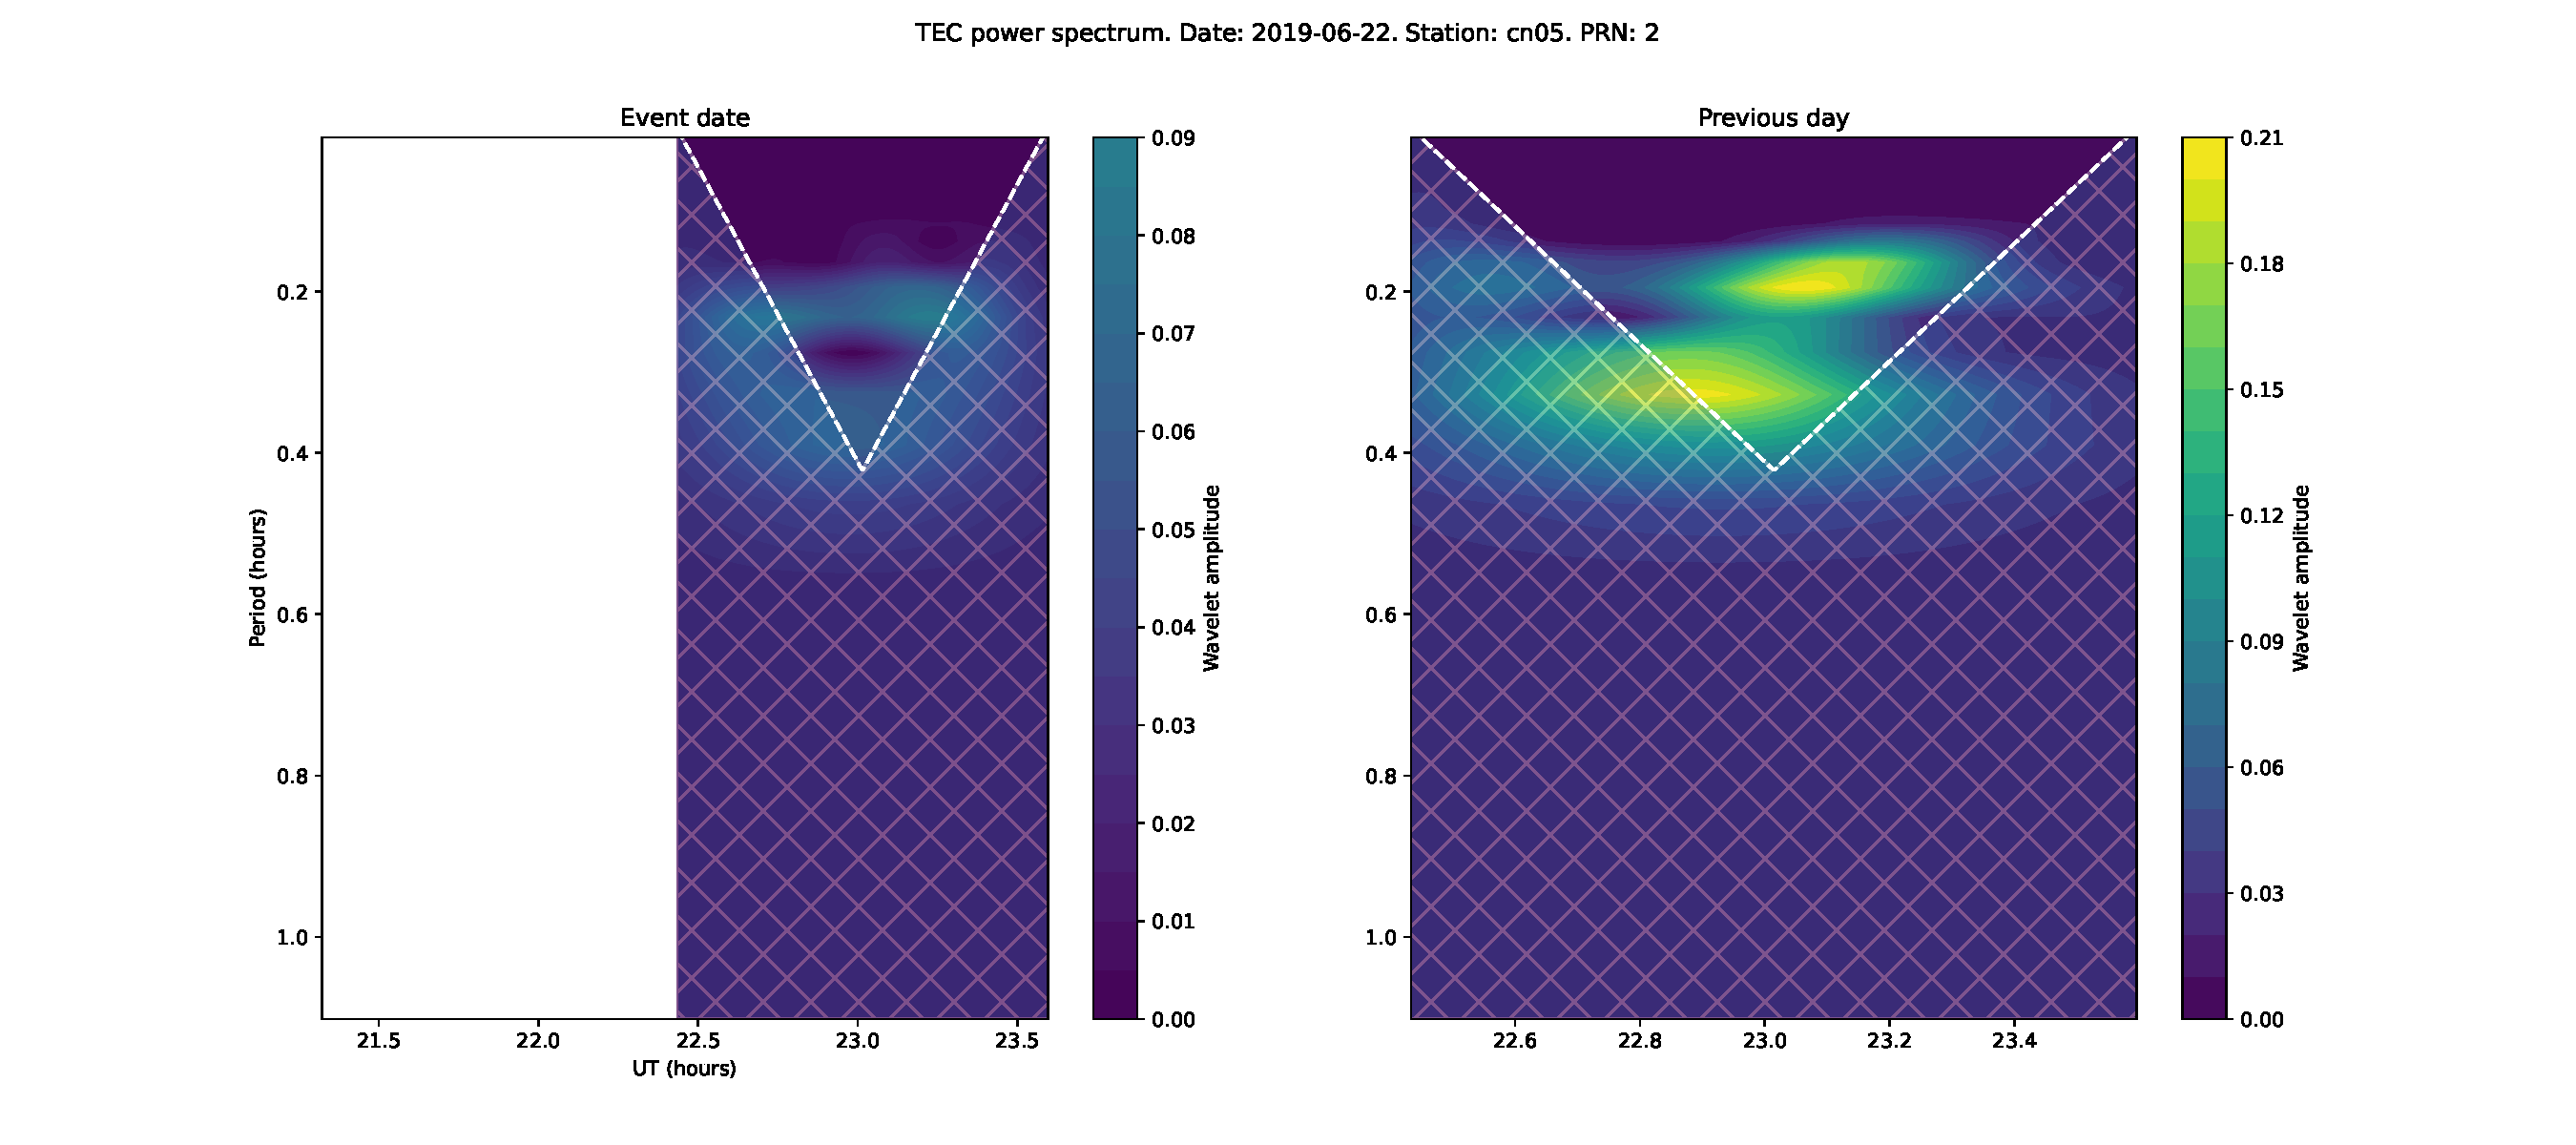
\includegraphics[width=0.5\linewidth]{../figures/cn05-PRN2-contour}  & 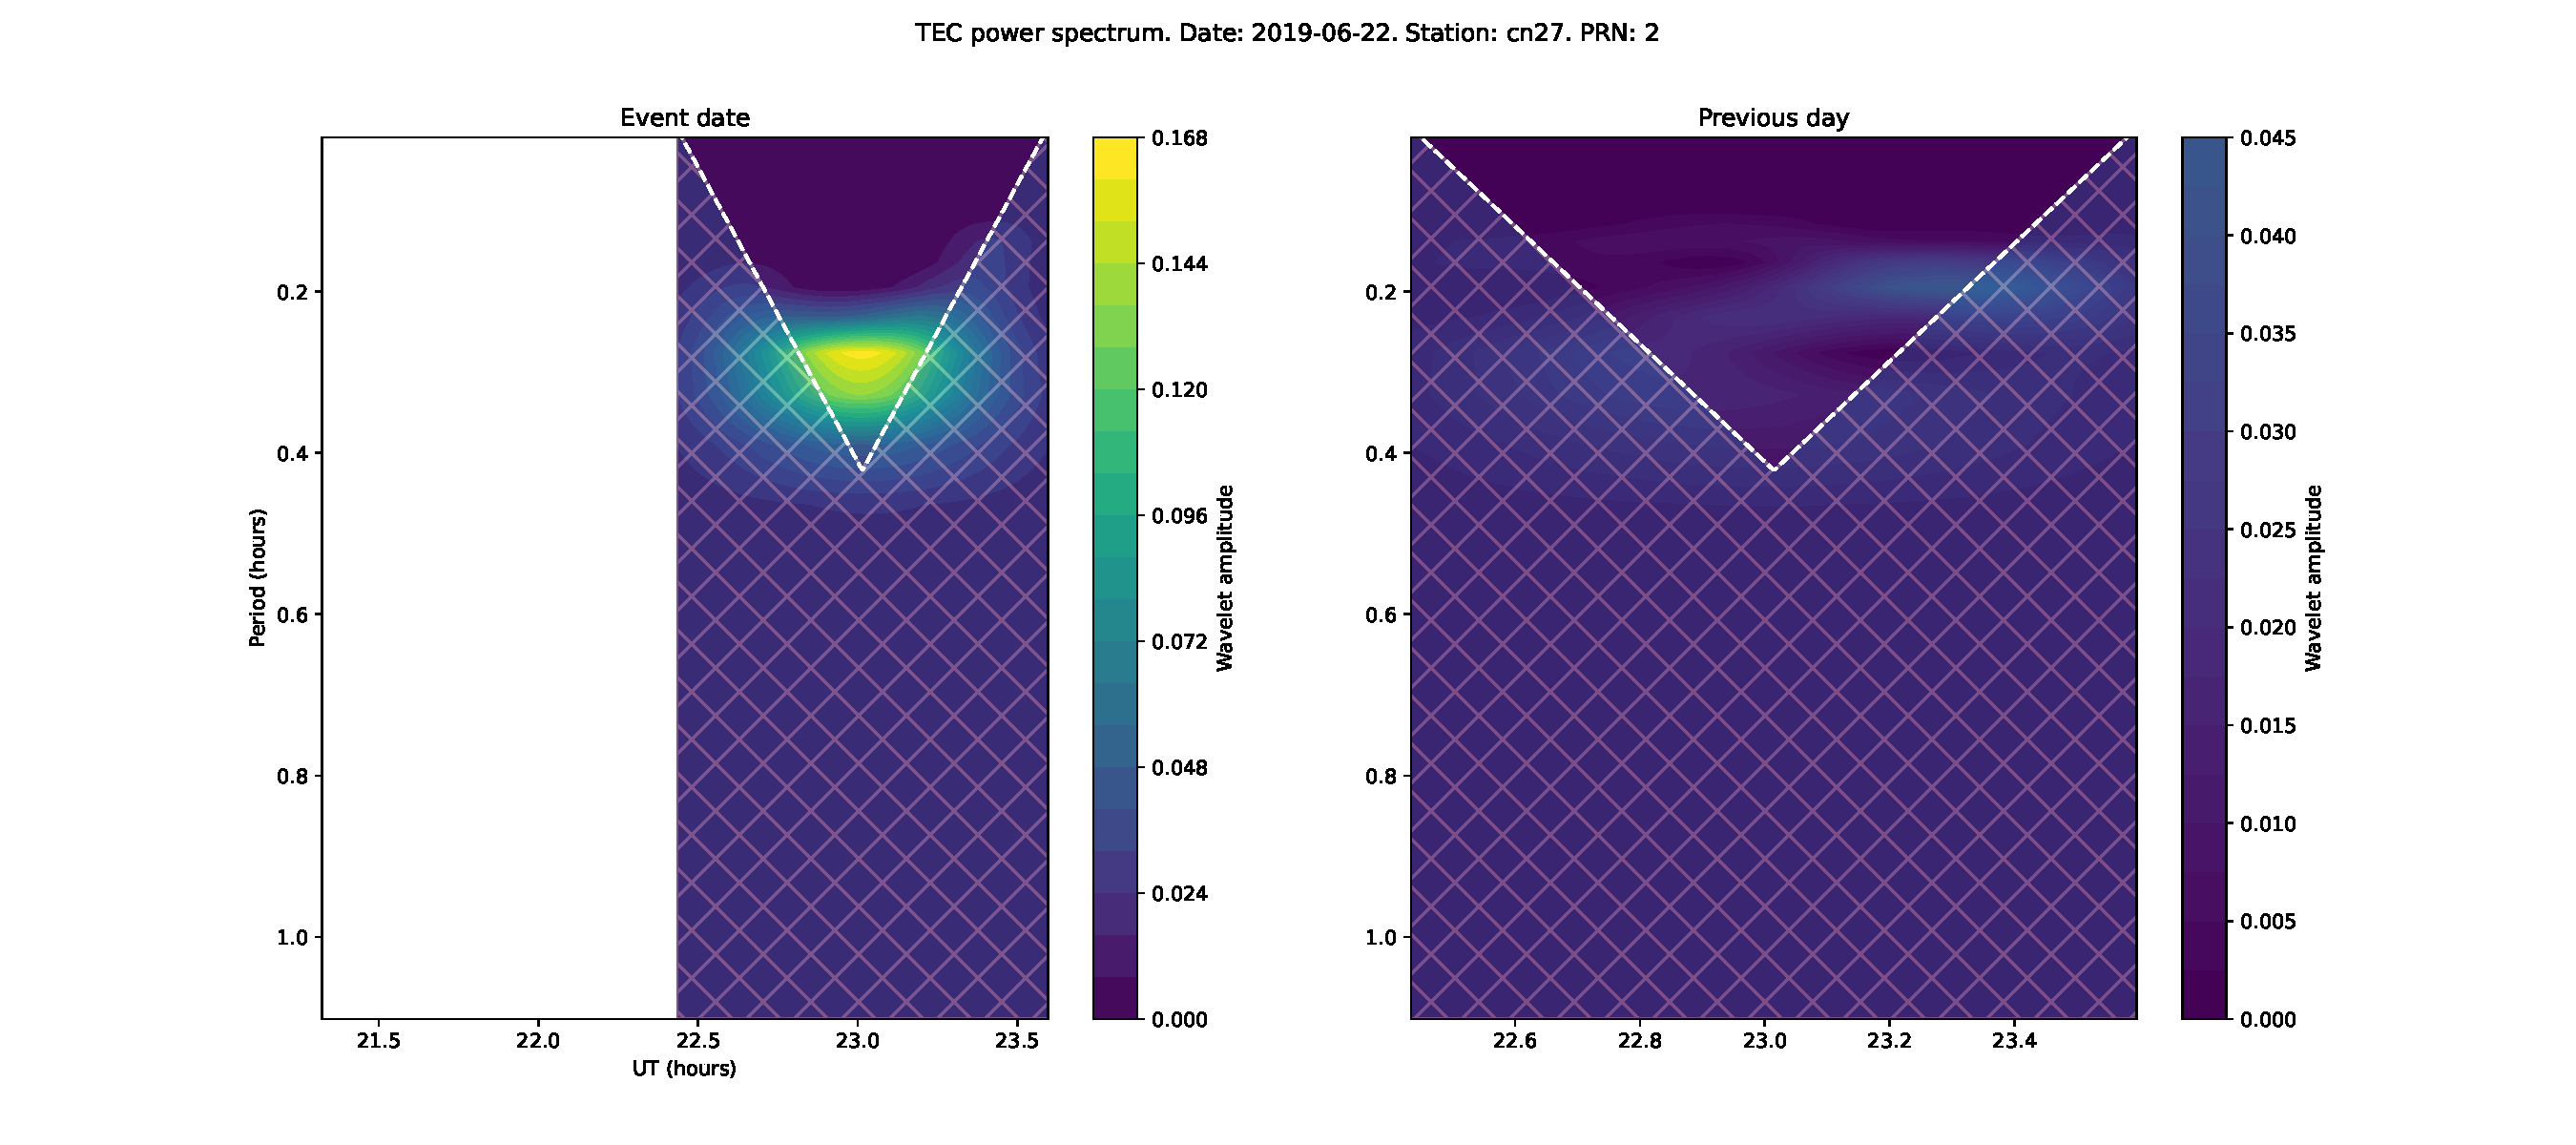
\includegraphics[width=0.5\linewidth]{../figures/cn27-PRN2-contour}\\
  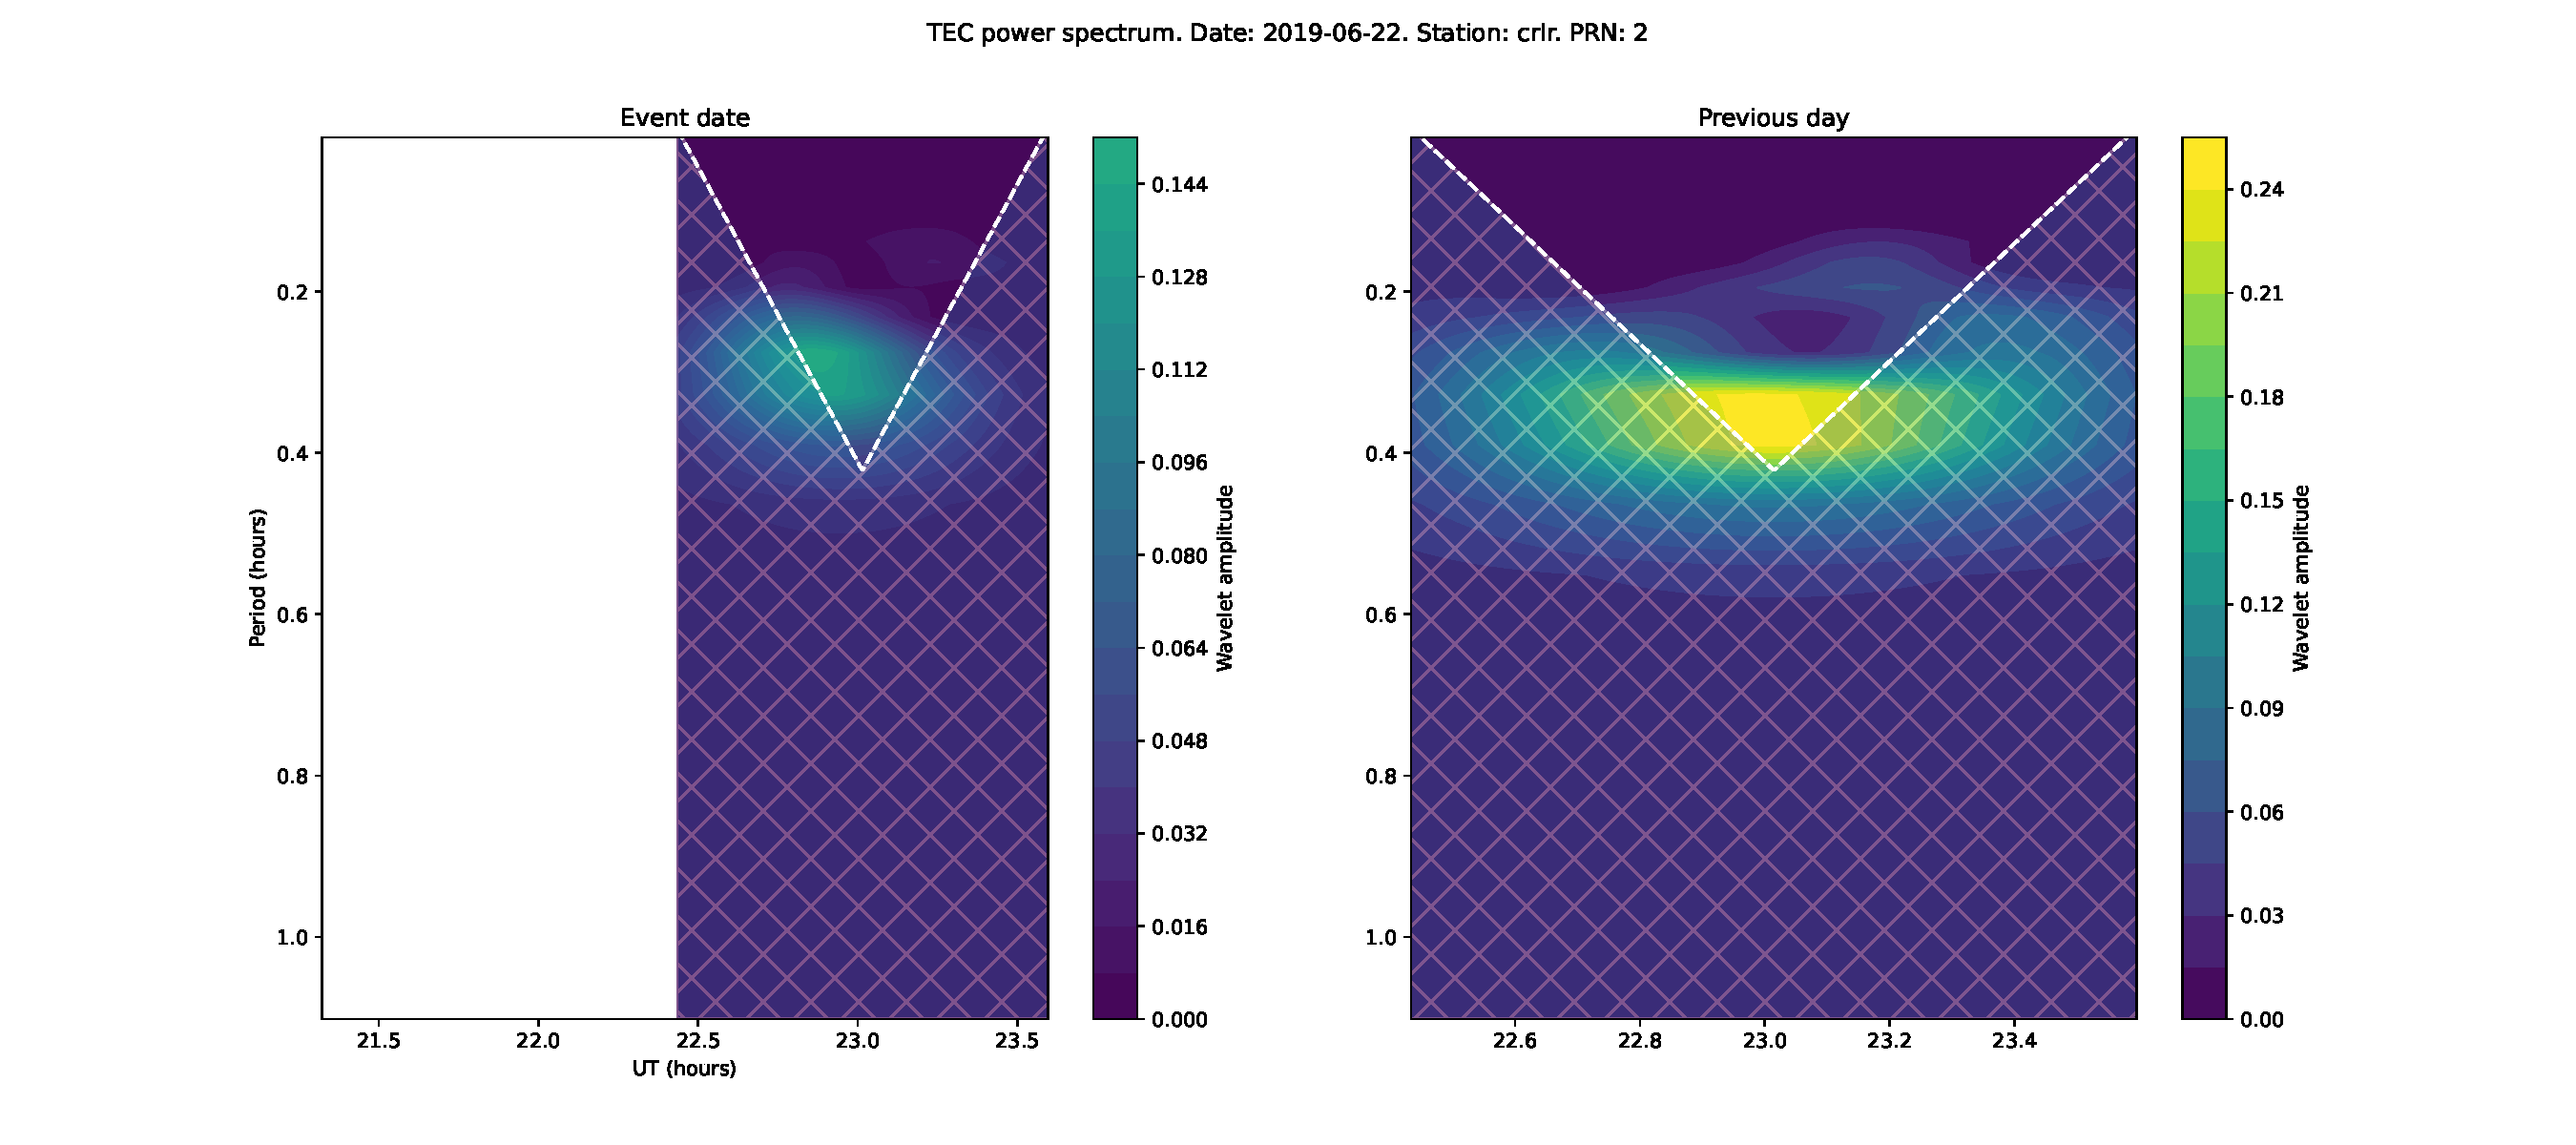
\includegraphics[width=0.5\linewidth]{../figures/crlr-PRN2-contour}  & 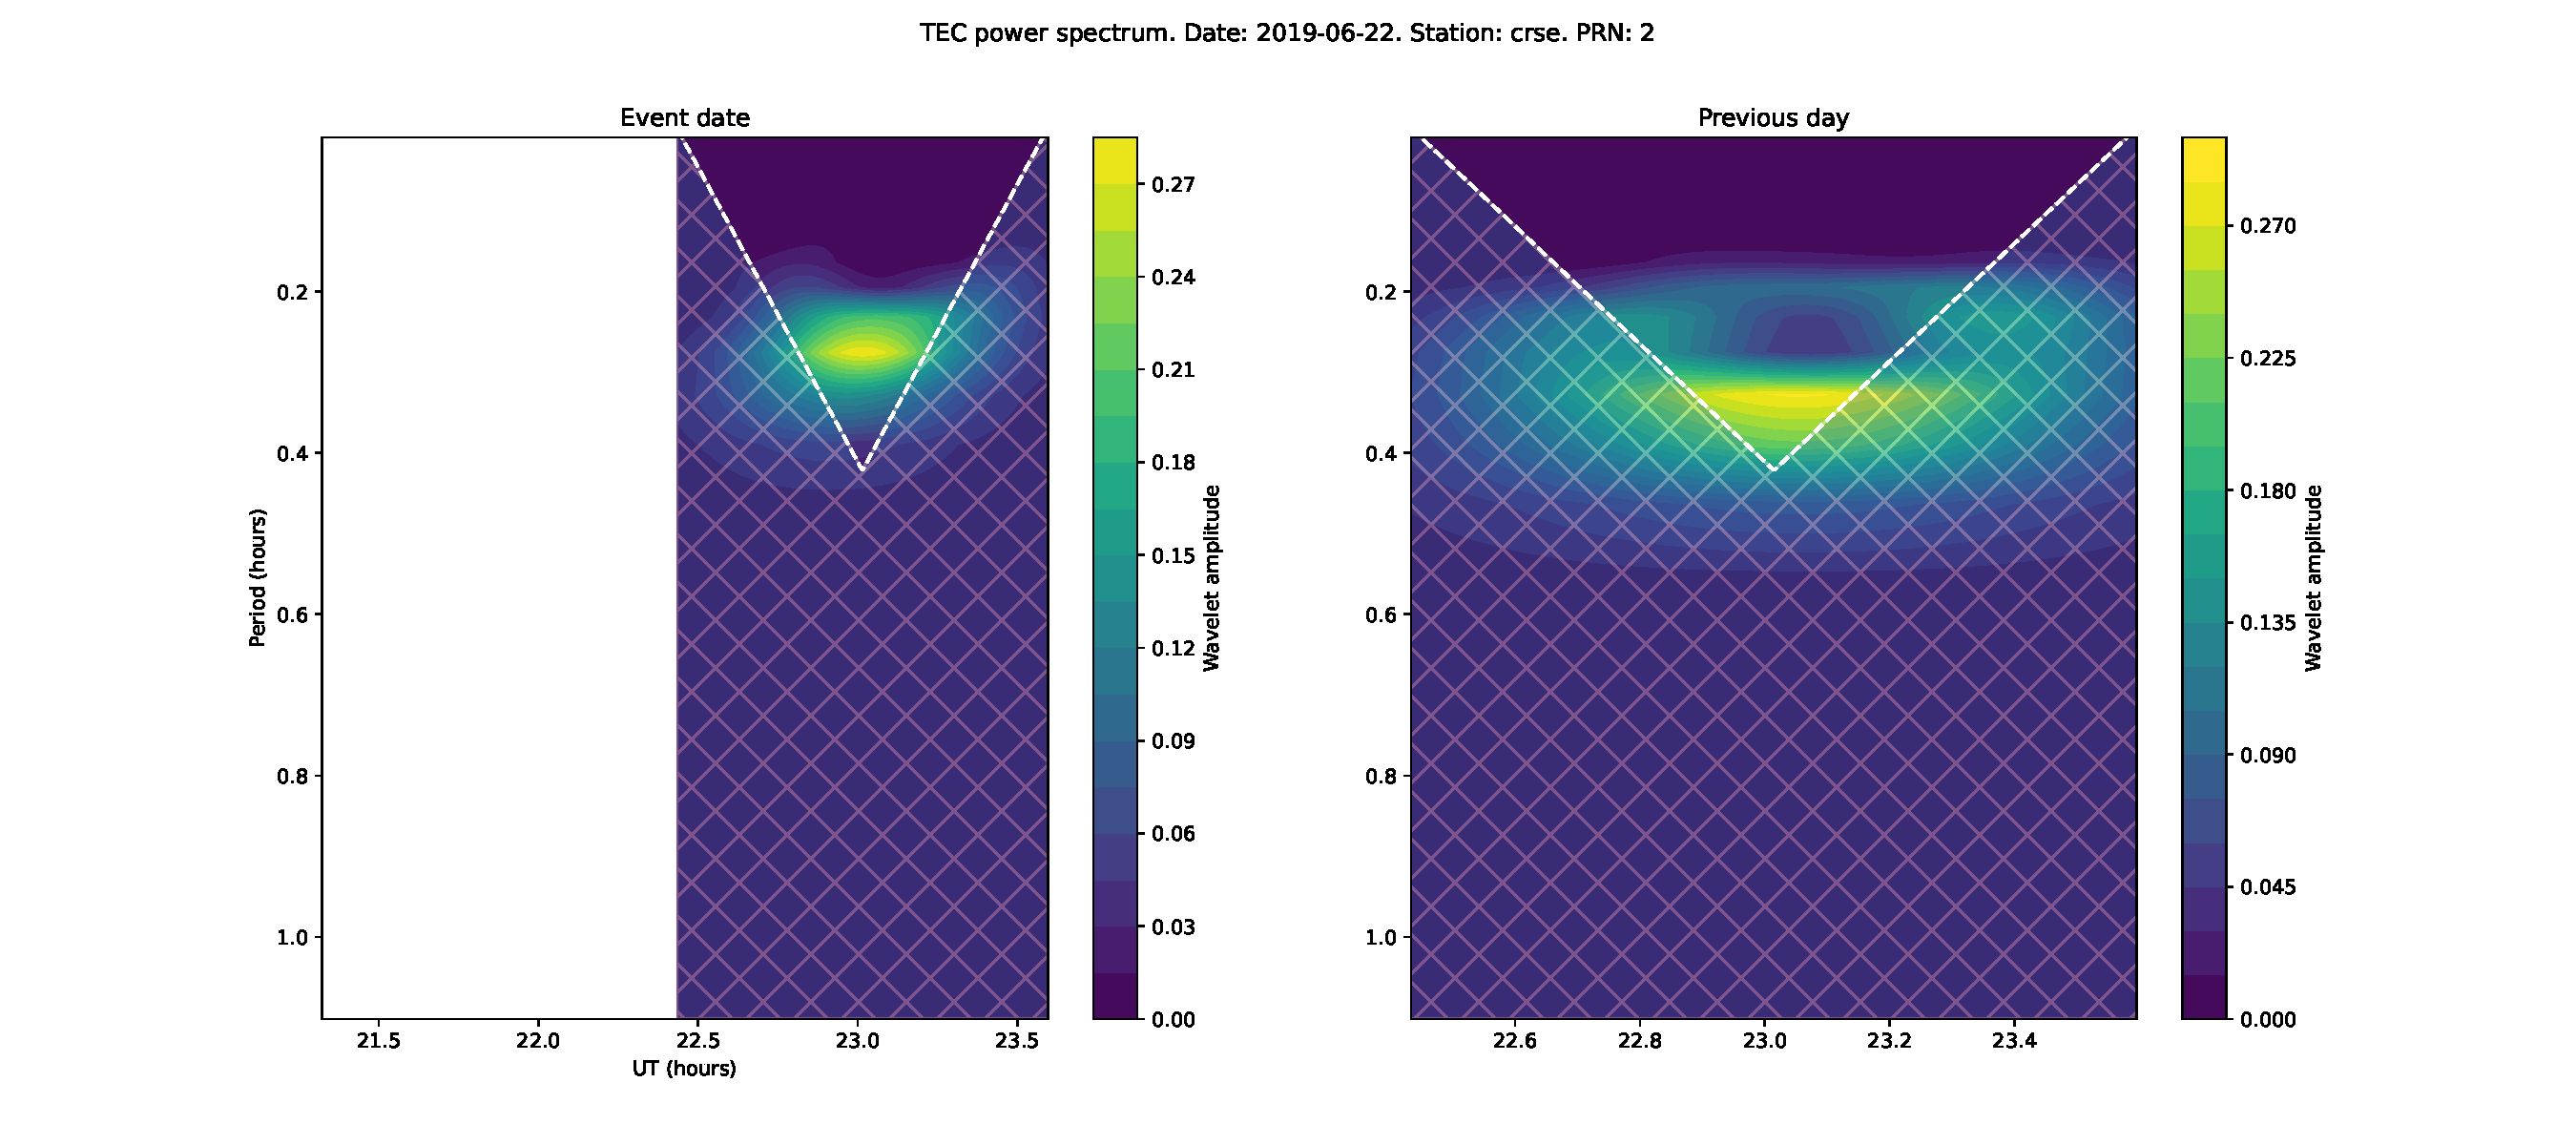
\includegraphics[width=0.5\linewidth]{../figures/crse-PRN2-contour}
  \end{tabular}
  \label{fig:power-spectrums}
  \caption{Examples of power spectrums for event USG-09, PRN 2. Top left: Station CN05. Top Right: Station CN27. Bottom left: station CRLR. Bottom right: station CRSE. In each figure the left panel corresponds to the event day and the right panel corresponds to the previous day of the event. The white dashed lines correspond to the Cone of Influence, where all the wavelet spectrum below is subject to error.}
\end{figure*}

  
